% Experimental evaluation
\section{ Experimental Evaluation} 

We ran experiments on real world datasets to
evaluate the performance of the algorithm. All the experiments were run
on an 4GB Intel Core i7 machine with a clock speed of $2.67$ GHz running
Ubuntu Linux 10.04. The code was written in C++ and 
compiled using g++ version $4.4$ with -O3
optimization flag. The default number of random walks is $K=500$.

\begin{comment}
\begin{table}[!h]
  \centering
    \begin{tabular}{|c|c|c|c|c|}
      \hline
      Dataset & $|V|$ & $|E|$ & $|\Sigma|$ & \small{Preprocessing time(sec)} \\
      \hline
      CMDB & $10466$ & $15122$ & $84$ & $329.31$ \\
      SCOP & $39256$ & $154328$ & $20$ & $17.377$ \\
      PPI & $4950$ & $16515$ & $4950$ & $339.45 $\\
      %Synthetic & $2755$ & $5002$ & $60$ \\
	  \hline
    \end{tabular}
    \caption{Dataset Properties}
	\label{tab:db}
\end{table}
\end{comment}


\begin{figure}[!h]
\centering
\subfloat[Dataset Statistics] {
	\label{subfig:dataset}	
	\begin{tabular}{|c|c|c|c|c|}
	\hline
		Dataset & $|V|$ & $|E|$ & $|\Sigma|$ & \small{Preprocessing time(sec)} \\
		\hline
		CMDB & $10466$ & $15122$ & $84$ & $329.31$ \\
		SCOP & $39256$ & $154328$ & $20$ & $17.377$ \\
		PPI & $4950$ & $16515$ & $4950$ & $339.45 $\\
		%Synthetic & $2755$ & $5002$ & $60$ \\
		\hline
		\end{tabular}
} \\
\subfloat[Maximal Pattern Statistics] {
	\label{subfig:maxpat_stats}
	\begin{tabular}{|c|c|c|c|}
	\hline
		Dataset & $|V|$ & $|E|$ & Degree\\
		\hline
		CMDB & $11$ & $12.24$ & $2.223$\\
		SCOP & $5.965$ & $6.725$ & $2.225$\\
		PPI & $6.453$ & $5.956$ & $1.655$\\
		%Synthetic & $2755$ & $5002$ & $60$ \\
		\hline
		\end{tabular}
}
  \caption{ \protect\subref{subfig:dataset}: Input graph statistics, 
    \protect\subref{subfig:maxpat_stats}: Maximal pattern statistics (the numbers
    shown are average values).
  }
  \label{fig:stats}
\end{figure}

\subsection{Configuration Management Database\\ (CMDB)} 

A CMDB is used to manage and query the IT infrastructure of an
organization. It stores information about the so-called configuration
items (CIs) -- servers, software, running processes, storage systems,
printers, routers, etc. As such it can be considered to be a single
large multi-attributed graph, where the nodes represent the various CIs
and the edges represent the connections between the CIs (e.g., the
processes on a particular server, along with starting and ending times).
Mining such graphs is challenging because they are large, complex,
multi-attributed, and have many repeated labels.  We used a real-world
CMDB graph for a large multi-national corporation (name not revealed due
to non-disclosure issues) from HP's Universal Configuration Management
Database (UCMDB).  Table~\ref{tab:db} shows the size of the CMDB graph. 


\smallskip\noindent{\textit{Cost Matrix}:} 
The set of labels in a CMDB form a
hierarchy which can be obtained from HP's UCMDB. In the absence of
domain knowledge, one way to obtain a cost matrix is by assigning low
costs for pairs of labels that share many ancestors in the hierarchy and
high costs otherwise. The algorithm is general in that it doesn't depend
on how the label matching costs are assigned or the range of these
values.  Consider any two labels $l_1$, $l_2$ and their corresponding
paths $p_1$, $p_2$ to the root node in the hierarchy.  We first define
the similarity between the labels to be proportional to the number of
common labels in $p_1 \cap p_2$, as follows
\begin{equation*}
  sim(l_1,l_2) =  \frac{|p_1 \cap p_2|}{2} \times 
  \left(\frac{1}{|p_1|} + \frac{1}{|p_2|}\right)
\end{equation*}
The cost of matching the labels is then 
$\matij{C}{l_1}{l_2} = 1 - sim(l_1,l_2)$.

\begin{figure}[!ht]
  \centerline{
    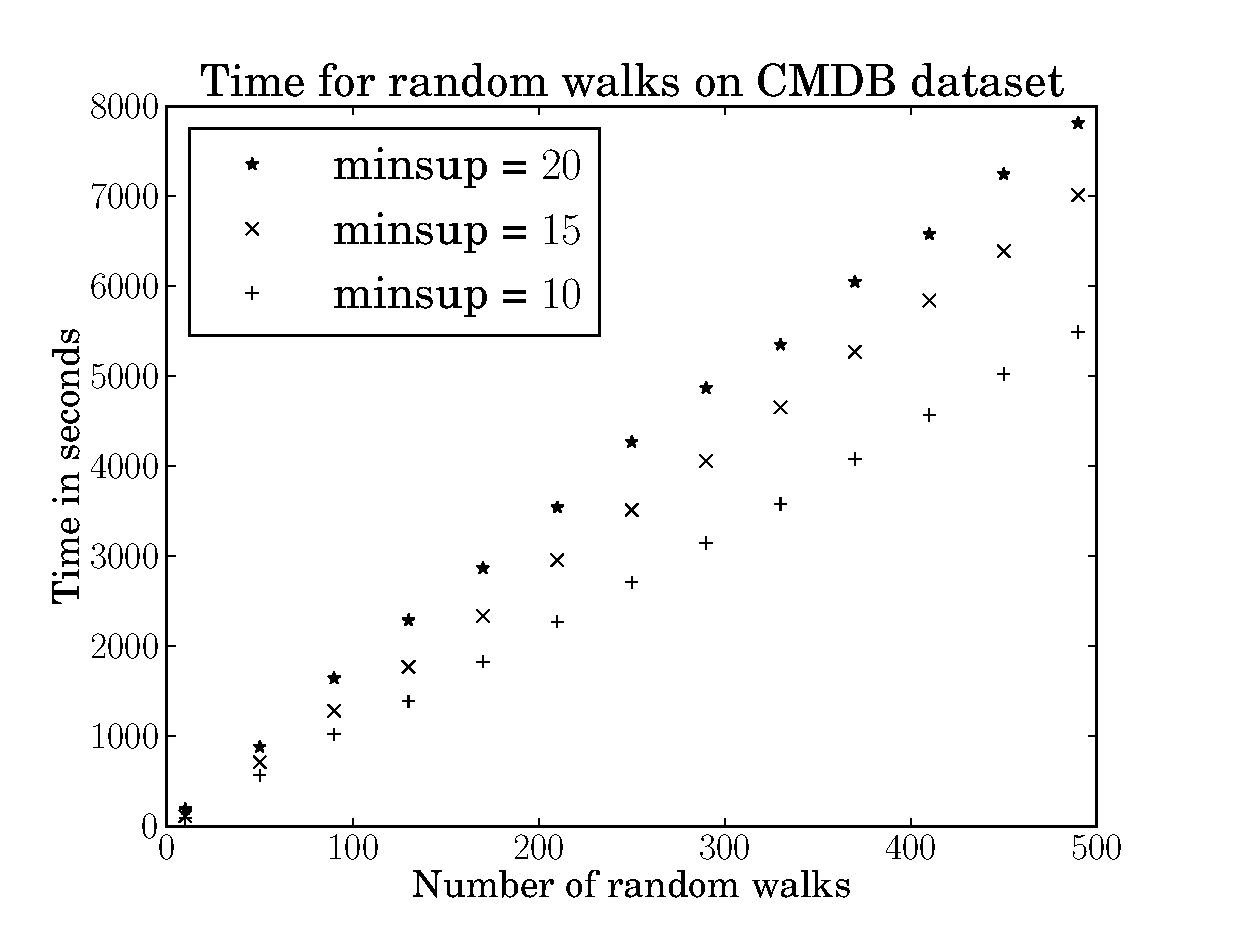
\includegraphics[width=2.5in]{ge.eps}
	}
    \caption{CMDB: Time for different values of
	$minsup$}
    \label{fig:ge}
\end{figure}


\smallskip\noindent{\textit{Results}:} Figure \ref{fig:ge} shows the
time for random walks for different values of $minsup$ and $\alpha =
0.5$. Interesting, and somewhat counter-intuitively, the time increases
for higher minimum support values.  The reason is that with higher
minimum support, the random walk in the search space goes through the
nodes that have a large number of embeddings and it takes more time to
enumerate a single pattern.

The running time results above include a particular optimization that we
applied for CMDB graphs, given the large multiplicities of the different
labels. For such graphs, the 
support computation procedure can be improved by computing the sets of
equivalent vertices, i.e., vertices that have the same neighborhood and
are indistinguishable. The representative set $R(u)$ of all equivalent
vertices are equal, and thus it has to be computed only once.  In
abstract algebra terms, such vertices belong to an orbit of the
automorphism group of the graph \cite{orbits}.  So, we can prune the
candidate representative sets of all the vertices in an orbit by
matching the labels of any vertex in the orbit with the labels of
vertices in the candidate set. Computing the orbits of an arbitrary
graph is a hard problem. Several heuristics have been proposed to
compute the orbits of a graph \cite{Everett}.  We use a simple heuristic
to find subsets of vertices, common ancestor leaves (CAL) that are
guaranteed to be in the same orbit. These are the subset of leaves that
have the same label and are connected to a common ancestor.  CAL is a
subset $S \subseteq \vg$, such that $\forall u \in S$ and the following
three properties hold true: i) $|N(u)|=1$, ii) $\exists v \in \vg$,
$(v,u) \in \eg$, and  iii) $L(u) = l$  for some $l \in \Sigma$.
An example of CAL is set of all vertices labeled ``9 $\times$ process'' in
figure \ref{fig:gepatsB}; here 9 is the multiplicity of that label. 
CAL sets have to be computed once for every
candidate and this step had negligible impact on the overall run time. 


\begin{figure}[!h]
    \centerline{
    \subfloat[Pattern $A$] {
	\label{fig:gepatsA}
      \scalebox{0.6}{
        \begin{pspicture}(-2,-0.5)(3,5)	
          \begin{psmatrix}[rowsep=1,colsep=1]
          \Toval[name=n4]{running\_software} & & \\
             \Toval[name=n1]{windows\_service} & \Tcircle[name=n2]{iis} &
            \Toval[name=n3]{iisftpservice}\\
            \Tcircle[name=n5]{nt} & & \\
            \Toval[name=n6]{ip\_address} & \Toval[name=n7]{webvirtualhost} &
            \Toval[name=n8]{iiswebsite}
            %\Toval[name=n1]{business\_application} & \Toval[name=n2]{windows\_service}\\
            %\Tcircle[name=n3]{nt} & \\
            %\Toval[name=n5]{sqlserver} & \Toval[name=n4]{process}\\
            %& \Toval[name=n6]{windows\_service $\times$ 8}
          \end{psmatrix}
          \ncline{n1}{n4}
          \ncline{n1}{n2}
          \ncline{n2}{n3}
          \ncline{n2}{n5}
          \ncline{n2}{n7}
          \ncline{n1}{n5}
          \ncline{n1}{n4}
          \ncline{n6}{n5}
          \ncline{n7}{n6}
          \ncline{n7}{n8}
          \ncline{n3}{n8}
        \end{pspicture}
      }
	  }}
	\centerline{
    \subfloat[Pattern $B$] {
	\label{fig:gepatsB}
      \scalebox{0.5}{
        \begin{pspicture}(-2,-1)(4,7)	
          \begin{psmatrix}[rowsep=1,colsep=1]
            & \Toval[name=n1]{9 $\times$ process} & & \Toval[name=n2]{ip\_address} \\
            & \Toval[name=n3]{windows\_service} & \Tcircle[name=n4]{nt} &
            \Toval[name=n5]{ip\_address} \\
            \Toval[name=n6]{iisftpservice} & \Tcircle[name=n7]{iis} & &
            \Toval[name=n8]{webvirtualhost} \\
            & & \Toval[name=n9]{iisappool} & \\
            & \Toval[name=n10]{iisftpservice} & & \Toval[name=n11]{iiswebsite} \\
          \end{psmatrix}
        \ncline{n1}{n4}
        \ncline{n2}{n4}
        \ncline{n3}{n4}
        \ncline{n5}{n4}
        \ncline{n6}{n7}
        \ncline{n3}{n7}
        \ncline{n8}{n7}
        \ncline{n7}{n9}
        \ncline{n11}{n9}
        \ncline{n11}{n8}
        \ncline{n7}{n10}
        \ncline{n10}{n11}
        \ncline{n5}{n8}
        \end{pspicture}
      }
	  }}
    \caption{CMDB: Approximate Patterns}
    \label{fig:gepats}
  \end{figure}

\smallskip\noindent{\textit{Example Patterns}:}
Figure \ref{fig:gepats} shows maximal approximate
patterns from the real world CMDB graph. Both these patterns show
typical ``default'' 
configurations of the IT infrastructure in this company. They show the
connection between some services running on an NT server, and also the
web/ftp services.


\begin{figure}
    \centering
    \scalebox{0.6}{
    \begin{pspicture}(0,0)(3,5)
          \begin{psmatrix}[rowsep=1,colsep=1]
          & \Toval[name=n1]{running\_software} & \\
          \Toval[name=n2]{EnrichActImpl} & & \Toval[name=n3]{process}\\
          \Toval[name=n4]{process} & \Toval[name=n5]{nt} &
          \Toval[name=n6]{ip\_address}\\
          & \Toval[name=n7]{$8 \times process$} & \\
          \end{psmatrix}
          \ncline{n1}{n2}
          \ncline{n2}{n3}
          \ncline{n2}{n4}
          \ncline{n2}{n5}
          \ncline{n4}{n5}
          \ncline{n5}{n6}
          \ncline{n5}{n3}
          \ncline{n5}{n1}
          \ncline{n5}{n7}
    \end{pspicture}
    }
    \caption{Complete Enumeration Expensive}
    \label{fig:geex}
\end{figure}

To show the effectiveness of the pruning based on labels, we compared
the time taken to enumerate a single maximal pattern in $CMDB$ database.
We compared the time with and without label-based pruning.
Both the methods terminated the random walk with the maximal pattern
shown in Figure~\ref{fig:geex}.  
However, the total time taken to enumerate the pattern
without using any derived label is $18306$ secs whereas by using the
\combined label the total time reduced to only $15.5776$ secs. The huge
difference between the times arises due to the multiplicity effect in
$CMDB$ graphs.  



\subsection{Protein Structure Dataset (SCOP)}
SCOP (\url{scop.mrc-lmb.cam.ac.uk/scop/}) 
is a hierarchical classification of proteins based on structure
and sequence similarity. The four levels of hierarchy in this
classification are: class, fold, superfamily and family.  The $3D$
structure of a protein can be represented as an undirected graph with
the vertex labels being the amino acids, with an edge connecting two
nodes if the distance between the 
3D coordinates of the two amino acids (their
$\alpha$-Carbon atoms) is within a threshold (we use 7 Angstroms).
We constructed a database of
$100$ protein structures belonging to $5$ different families with $20$
proteins from each family. 
We chose the proteins from different levels in the SCOP hierarchy, and
we also focused on large proteins (those with more than 200 amino
acids). 
The 3D protein structures were downloaded from the
protein data bank (\url{http://www.rcsb.org/pdb}).  The database
can be considered as a single large graph with $100$ connected
components. 
For the SCOP dataset, the support is redefined as 
the number of proteins containing the pattern, i.e., 
even if a protein contains multiple embeddings we count them only once for the support.

\smallskip\noindent{\textit{Cost Matrix}:}
Since there are 20 different amino acids, we need a $20 \times 20$ cost
matrix. BLOSUM62~\cite{HH92} is a commonly used substitution matrix for aligning protein
sequences.  The $i,j$ entry in BLOSUM denotes the log-odd score
of substituting the amino acids $a_i$ and $a_j$, defined as
\begin{equation*}
    \label{eq:blosum}
    \matij{B}{i}{j} = \frac{1}{\lambda} 
	\log\frac{p_{ij}}{f_i \cdot f_j}
\end{equation*}
where $p_{ij}$ denotes the probability that  $a_i$ can be
substituted by $a_j$; 
$f_i$, $f_j$ denote the prior probabilities for observing the 
amino acids; and $\lambda$ is a constant. We compute $f_i$ and $f_j$
from the database, and then reconstruct $p_{ij}=f_if_j e^{\lambda
B_{i}}$. Next, we define the pair-wise amino acid cost matrix as
$\matij{C}{i}{j} = 1-\frac{p_{ij}}{p_{ii}}$, which ensures that
the diagonal entries are $\matij{C}{i}{i} =0$.

\begin{figure}[!ht]
	\centerline{
    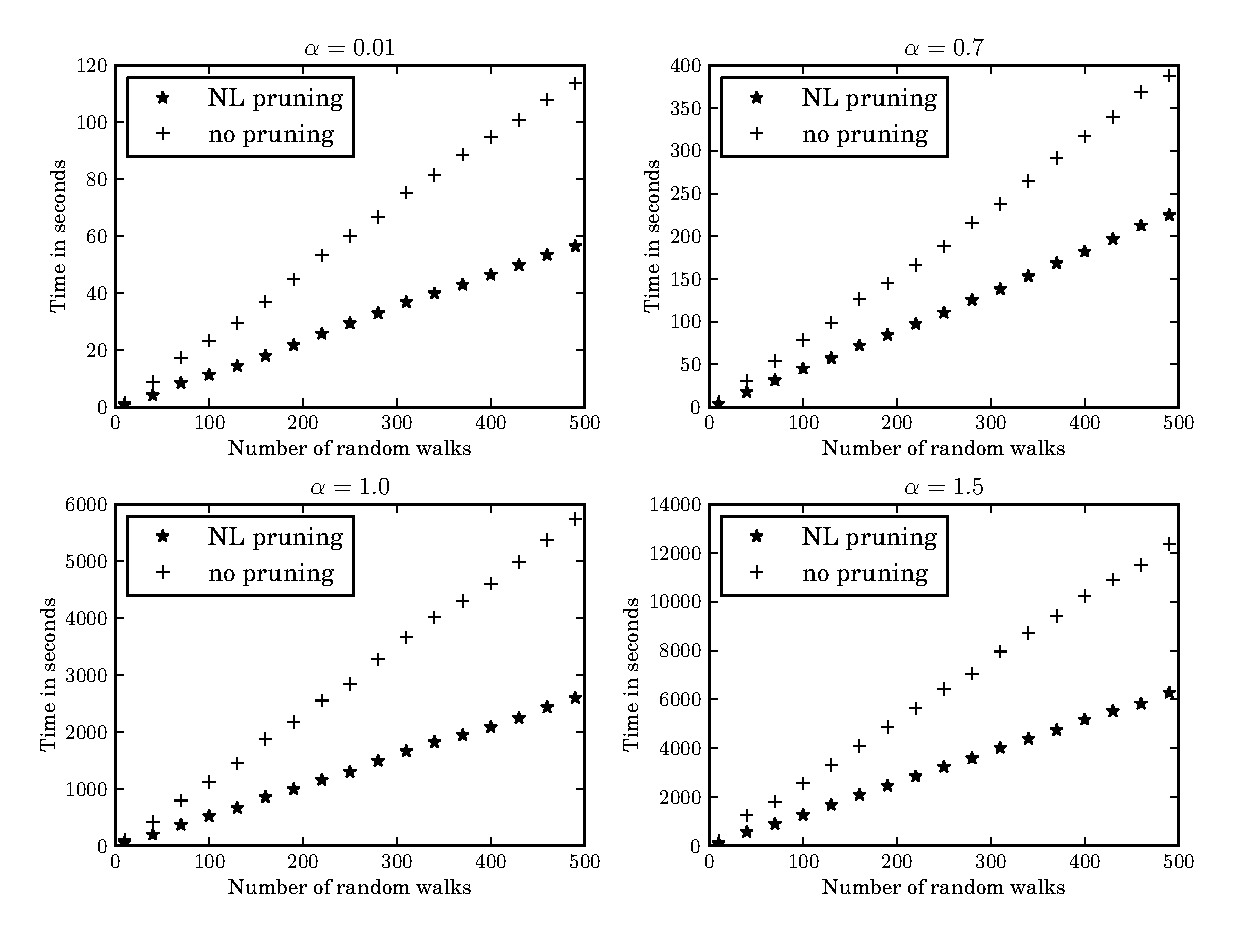
\includegraphics[width=3in]{5F20P.eps}
	}
	\caption{SCOP: Effect of $\alpha$ (increasing in 
	clockwise order from top right)}
    \label{fig:5F20P}
\end{figure}

\begin{figure}[!ht]
  \centerline{
    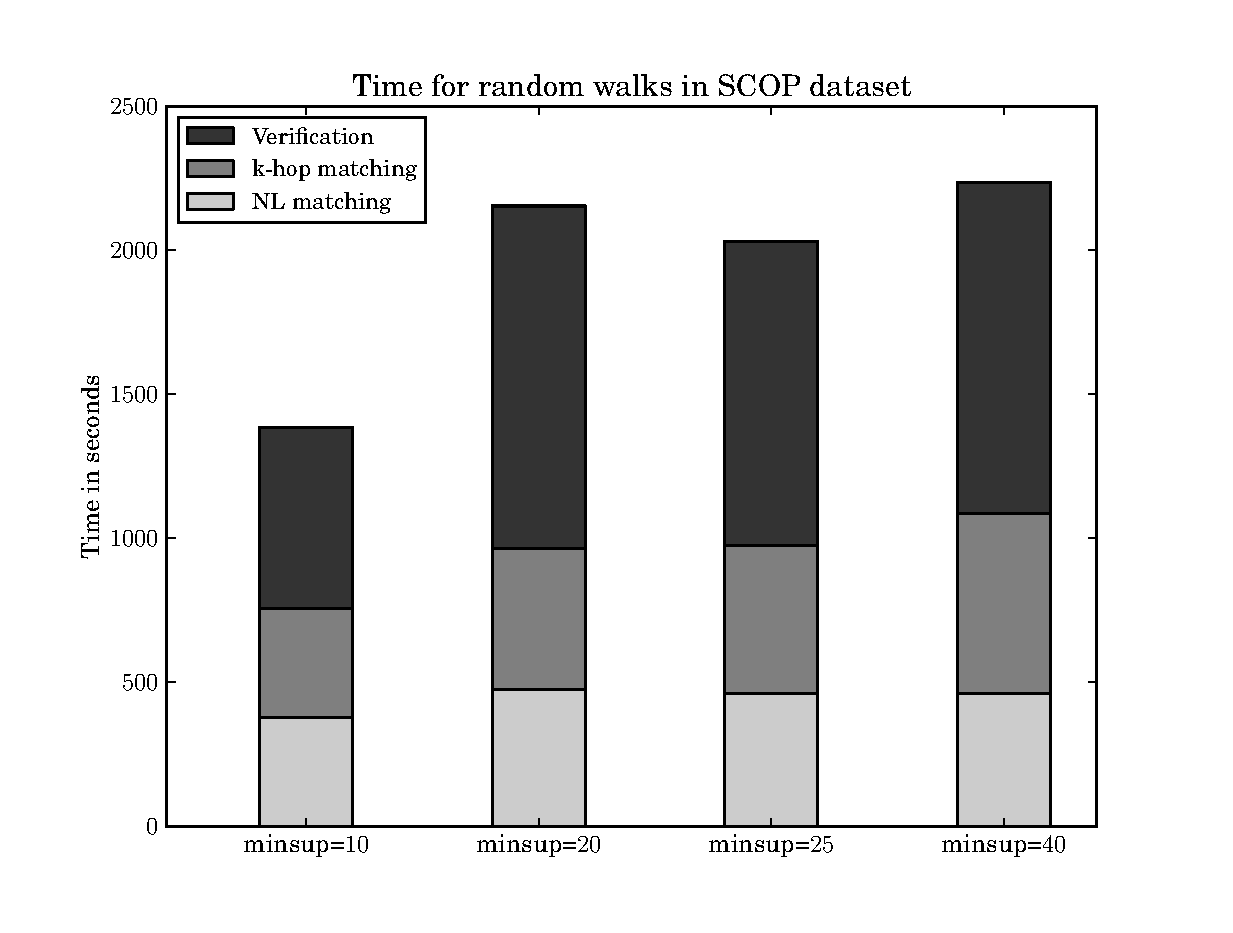
\includegraphics[width=2.5in]{scop_minsup.eps}
	}
	\caption{SCOP: Effect of $minsup$}
    \label{fig:5F20P_ft}
\end{figure}


\smallskip\noindent{\textit{Results}:}
Figure \ref{fig:5F20P} shows the time taken for enumerating approximate
maximal patterns for different values of $\alpha$ (with fixed $minsup =
20$). The plots show the time for random walks with and without the
label pruning. It can be seen that by using the label-based pruning the
time for random walks reduces significantly (by over 100\%).  As
expected, the time increases as the values of $\alpha$ increases, since
the number of isomorphisms clearly increases for a more relaxed (larger)
cost threshold.  When $\alpha = 0.01$, the patterns are exact as
$\matij{C}{i}{j} > \alpha$ $,\forall i \neq j$.

Figure \ref{fig:5F20P_ft} shows the time taken for $K=500$ random walks
for various values of $minsup$, but with a fixed $\alpha = 0.7$. The bar
plot shows time spent in \khop matching (Hops), \ncl matching
(Neighbors) and pattern verification (Enumeration). In general, the time
increases as the $minsup$ increases because the representative sets
$R(u)$ become larger. However, there is no fixed trend as the total time
depends on the regions of pattern space that the random walk explores.

\begin{figure}[!ht]
  \centerline{
    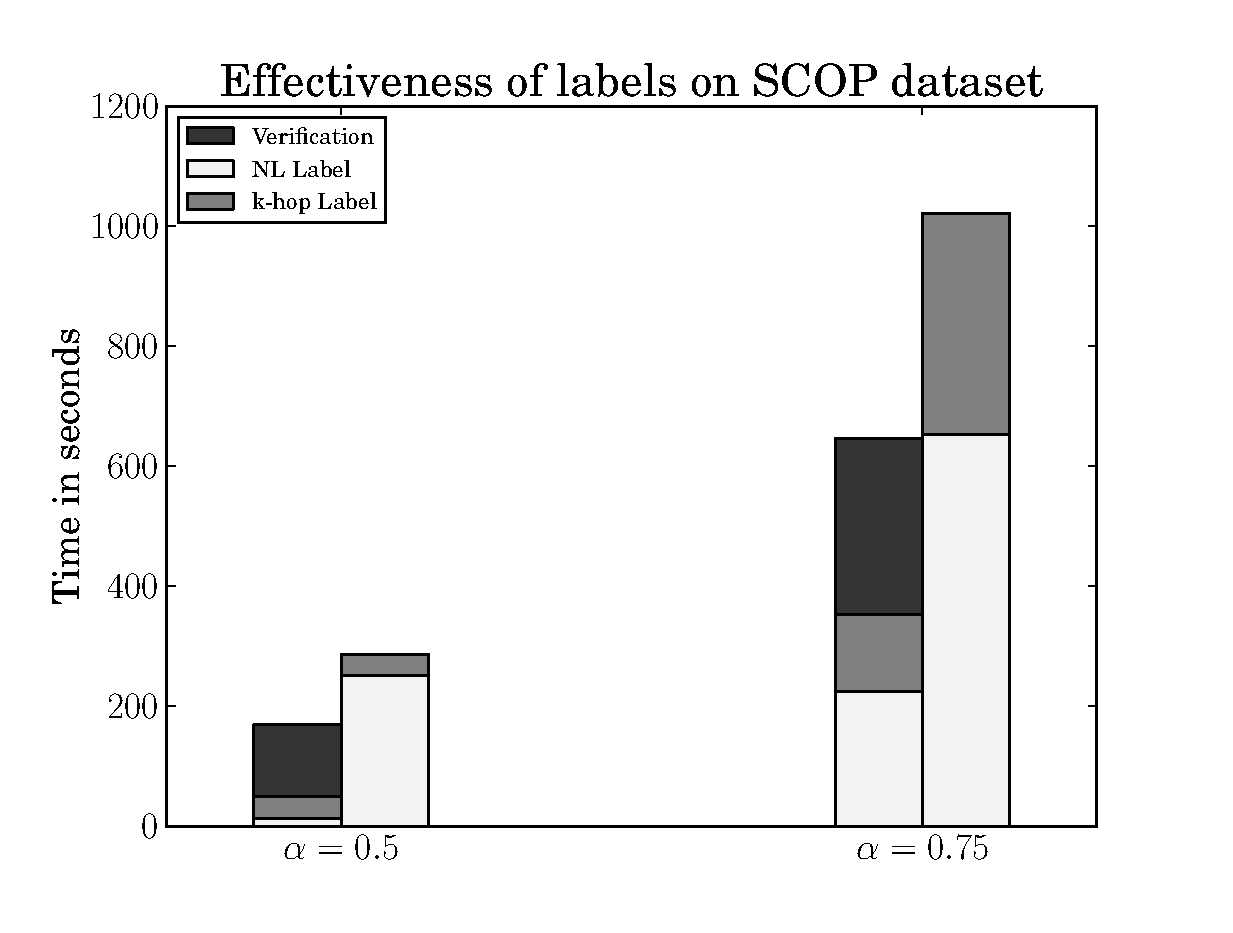
\includegraphics[width=2.5in]{scop_effectiveness.eps}
	}
	\caption{SCOP: Effectiveness of labels}
    \label{fig:D5F20P_eff}
\end{figure}

Figure~\ref{fig:D5F20P_eff} compares the effectiveness of the \combined
label (Neighbors) and \khop label (Hops) for different values of the
threshold $\alpha$ on the SCOP dataset.  For each value of $\alpha$, the
left bar shows the time with \combined label, whereas the right bar
shows the time using only the \khop label.  The \combined label clearly
reduces the time taken. In fact, it reduces the time for both the \khop
matching and the pattern verification steps, since \combined is very
effective in pruning the representative set.  This effect is best seen
for $\alpha = 0.75$, where the total time for the enumeration reduces
even though matching the neighbors takes more time compared to \khop
matching.  This shows the effectiveness of the \combined label versus
\khop label in isolation.

\begin{figure}[!ht]
  \centerline{
  \subfloat[Pattern $A$]{
    \label{fig:scopA}
    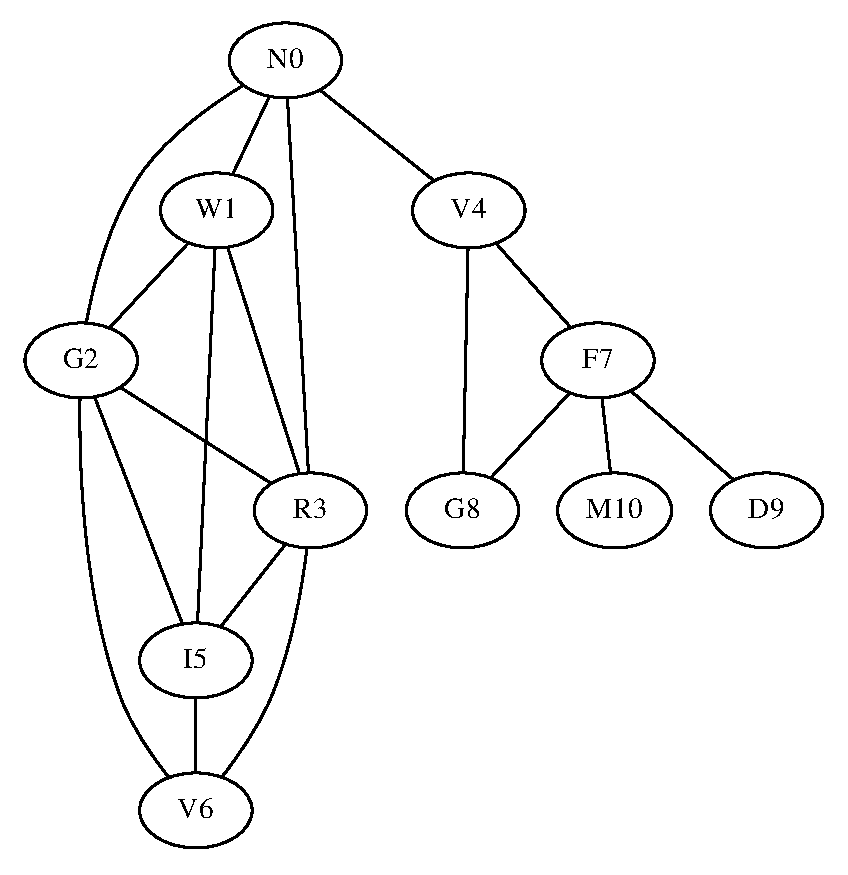
\includegraphics[width=1.5in,height=1.25in]{1ysw.pat.eps}
	}
  \subfloat[Pattern $B$]{
    \label{fig:scopB}
    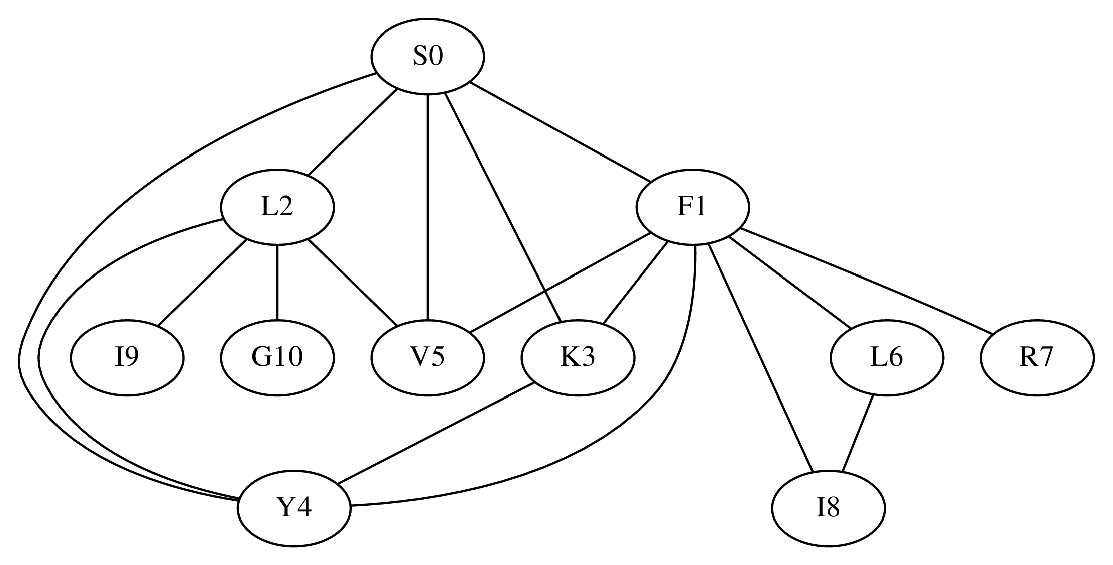
\includegraphics[width=1.5in,height=1.0in]{1r2e.pat.eps}
	}	
	}
	\centerline{
	\subfloat[Structural Motif $A$]{
    \label{fig:scopAS}
    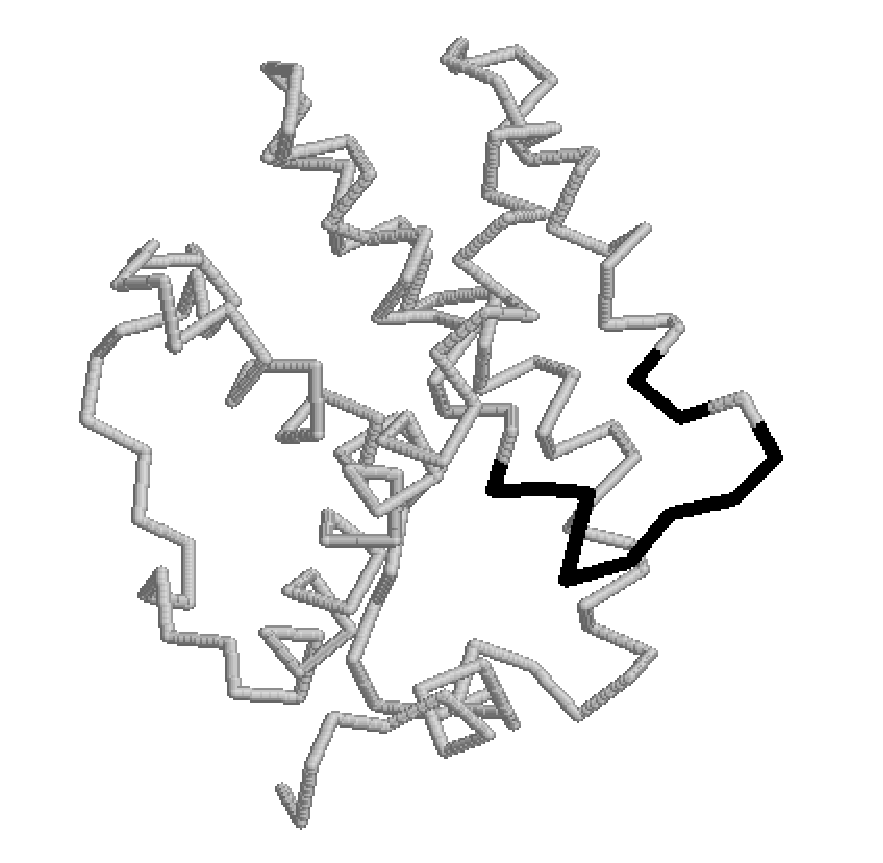
\includegraphics[width=1.5in,height=1.5in]{1ysw.eps}
	}
	\subfloat[Structural Motif $B$]{
    \label{fig:scopBS}
    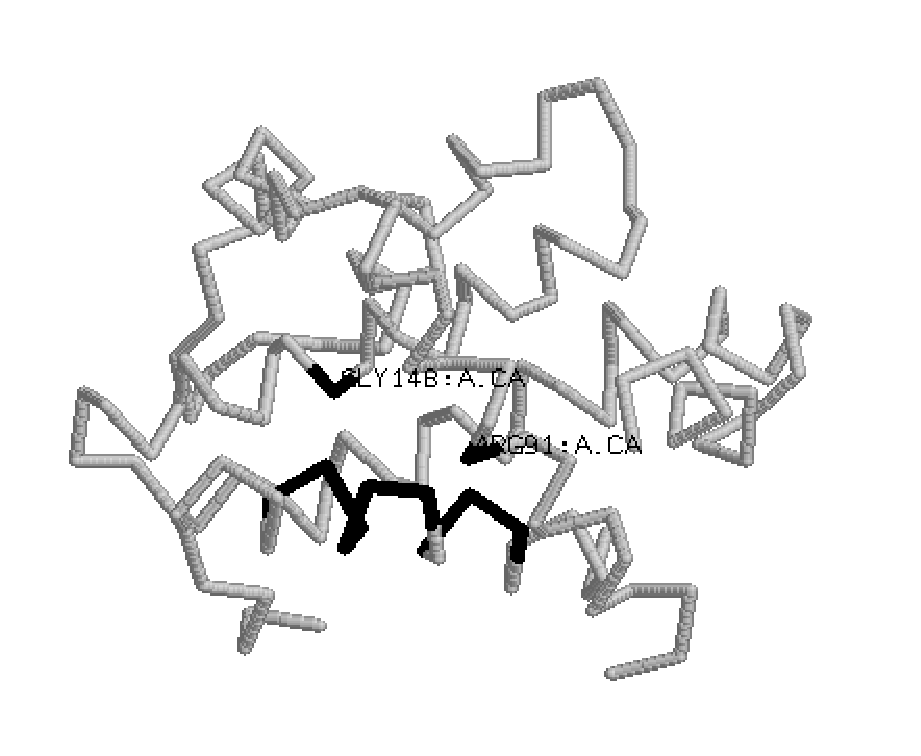
\includegraphics[width=1.5in,height=1.5in]{1r2e.eps}
	}
	}
	\caption{SCOP: Approximate Graph Patterns and their Structures}
	\label{fig:scoppats}
\end{figure}


\smallskip\noindent{\textit{Example Patterns}:}
Figure~\ref{fig:scoppats} shows examples of approximate protein graph
patterns and their corresponding 3D structure extracted from the SCOP
dataset.  For example, the graph in \ref{fig:scopA} appears in only one of
the families. This pattern occurs in 18 of the 20 members, and the
structure of one its occurrences, in protein PDB:1YSW, is shown in
\ref{fig:scopAS}. The common motif corresponds to the black colored
amino acids.  Another approximate pattern is shown in \ref{fig:scopB},
and its structure in PDB:1R2E is shown in \ref{fig:scopBS}; it has
support 19.  It is important to note that the cost of this isomorphism
is $C(\phi) = 0.4541$, indicating that exact isomorphism cannot find the
motif.

\subsection{Protein-Protein Interaction Network (PPI)} We ran
experiments on a yeast (Saccharomyces cerevisiae) PPI network. The list of
interacting proteins for yeast was downloaded from the DIP database
(\url{http://dip.doe-mbi.ucla.edu}). As seen in Table~\ref{tab:db}, the
PPI network has 4950 proteins and 16,515 interactions.  Unlike the other
datasets, each node in the PPI network essentially has a unique label,
which is the protein name.  

\smallskip\noindent{\textit{Cost Matrix}:} 
To construct the cost matrix for the protein network we consider the
similarity between the protein sequences for any two adjacent nodes.
Sequence similarity is obtained via the BLAST alignment
score~\cite{altschul90}, that returns the expected value (E-value) of
the match. A low E-value implies high similarity, thus we create a
binary cost matrix between the proteins by setting
$\matij{C}{p_i}{p_j} =0$ iff the proteins $p_i$ and $p_j$ have high
similarity, i.e., iff $E-value(p_i, p_j) \le \epsilon$. We empirically 
set $\epsilon = 0.003$.


\begin{figure}[!h]
	\centerline{
	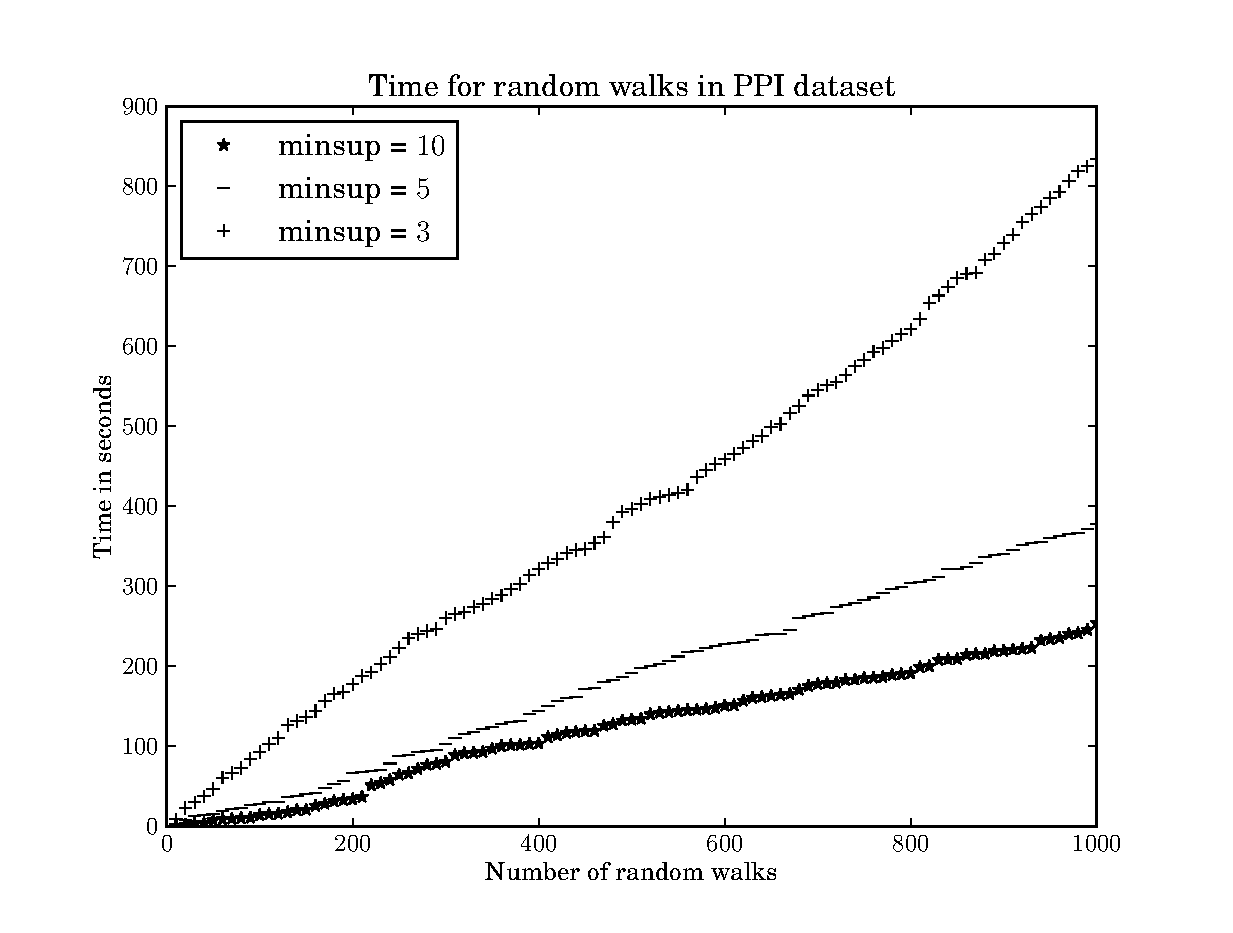
\includegraphics[width=2.5in]{ppi.eps}
	}
    \caption{PPI: Time for different values of $minsup$}
    \label{fig:ppiwalks}
\end{figure}

\smallskip\noindent{\textit{Results}:} Figure \ref{fig:ppiwalks} shows
the time for random walks in the yeast $PPI$ network for different values of
$minsup$.  It can be seen that the time for random walks decreases as
the support value increases.  One of the differences for the PPI graph
is that we do not utilize the \khop labels.  The complexity of matching
the \khop labels depends on the number of literals in the \khop label.
As each label(protein) is unique in the PPI graph, the number of
literals in the \khop label of a vertex $v$ in a PPI network is equal to
the number of vertices reachable in \khops. This increases the run time
for the \khop label matching.  Therefore, for mining PPI networks we use
only the \ncl labels.


\begin{figure}[!ht]
  \subfloat[Pattern $A$]{
    \label{fig:ppipatsA}
    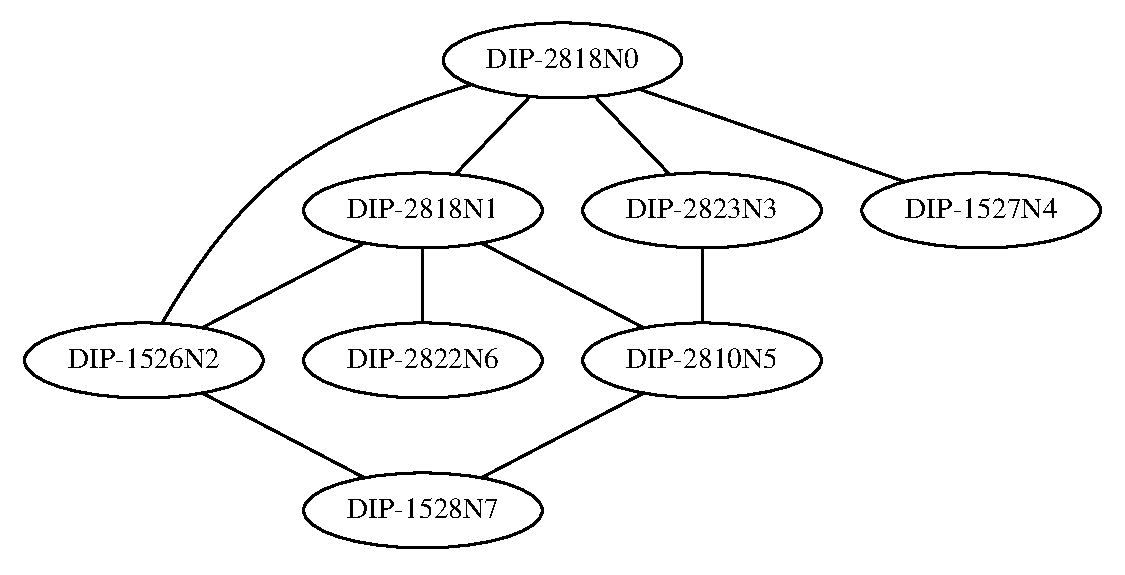
\includegraphics[width=2in]{ppipat2.eps}
	}\\
\subfloat[GO Terms for $A$]{
  % Table for the search space pruning
    \label{fig:ppipatsAT}
  \begin{tabular}{c|p{2in}}
GO Terms & Description\\
\hline
BP:0051603&      proteolysis involved in cellular protein catabolic
process\\
\hline
MF:0004298&      threonine-type endopeptidase activity\\
\hline
CC:0034515&      proteasome storage granule\\
  \end{tabular}
  %\label{subfig:match}
  } \\ 
  \subfloat[Pattern $B$]{
    \label{fig:ppipatsB}
    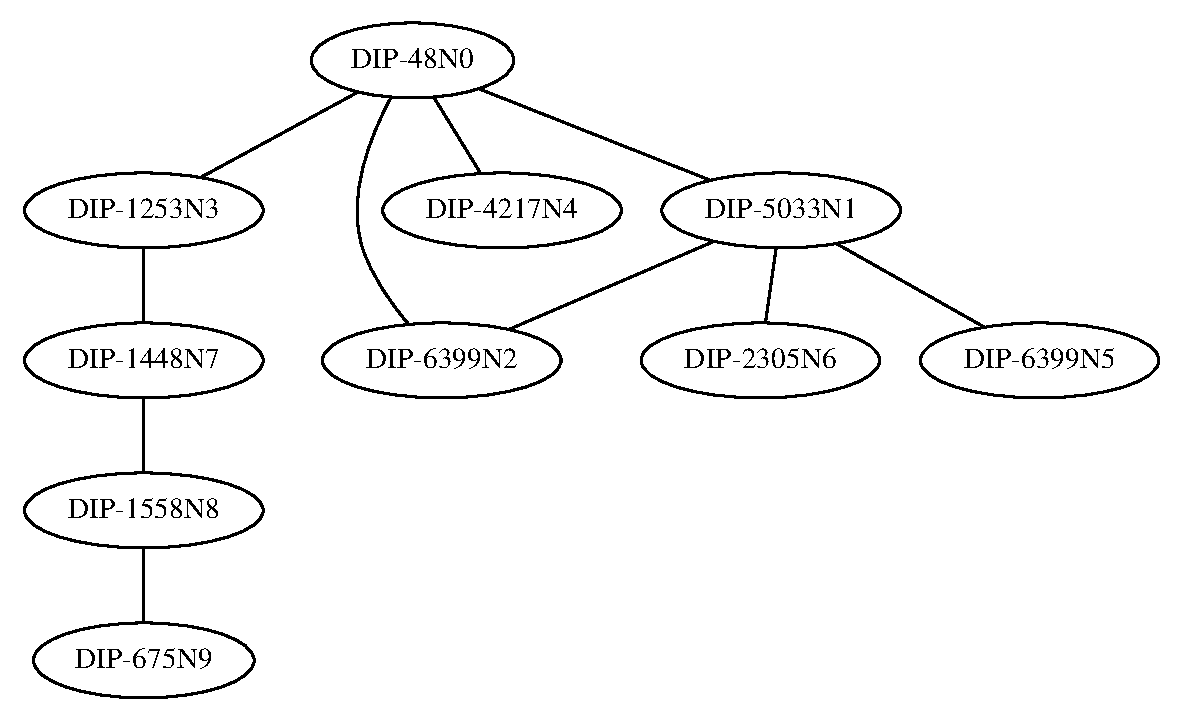
\includegraphics[width=2in]{ppipat1.eps}
	}\\
  \subfloat[GO Terms for $B$]{
    \label{fig:ppipatsBT}
  \begin{tabular}{c|p{2in}}
GO Terms & Description\\
\hline
BP:0004674  & protein serine/threonine kinase activity\\
\hline
MF:0016301   &   kinase activity\\
MF:0005524   &   ATP binding\\
  \end{tabular}
  }
    \caption{Approximate PPI Patterns and GO Enrichment}
    \label{fig:ppipats}
\end{figure}

\begin{comment}
\begin{figure}[!ht]
  \centerline{
  \subfloat[Pattern $A$]{
    \label{fig:ppipatsA}
    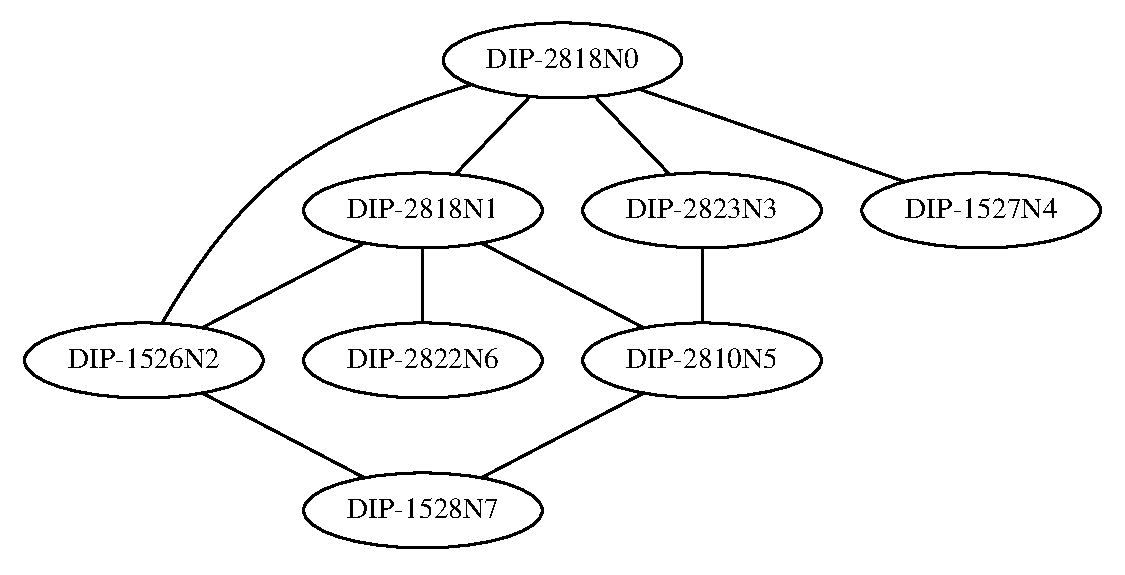
\includegraphics[width=2in]{ppipat2.eps}
	}}
	\centerline{
  \subfloat[GO Terms for $A$]{
    \label{fig:ppipatsAT}
  \small
  \begin{tabular}{c|p{2in}}
GO Terms & Description\\
\hline
BP:0051603&      proteolysis involved in cellular protein catabolic
process\\
\hline
MF:0004298&      threonine-type endopeptidase activity\\
\hline
CC:0034515&      proteasome storage granule\\
  \end{tabular}
  }}
  \centerline{
  \subfloat[Pattern $B$]{
    \label{fig:ppipatsB}
    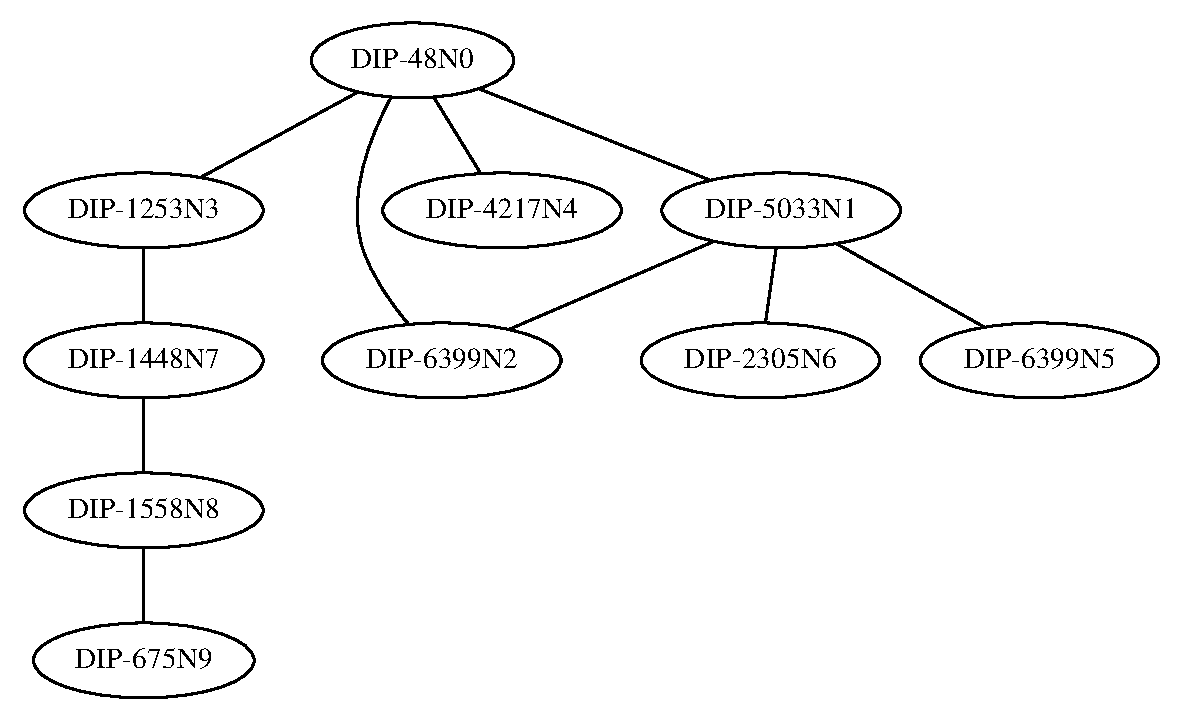
\includegraphics[width=2in]{ppipat1.eps}
	}}
	\centerline{
  \subfloat[GO Terms for $B$]{
    \label{fig:ppipatsBT}
  \small
  \begin{tabular}{c|p{2in}}
GO Terms & Description\\
\hline
BP:0004674  & protein serine/threonine kinase activity\\
\hline
MF:0016301   &   kinase activity\\
MF:0005524   &   ATP binding\\
  \end{tabular}
  }}
    \caption{Approximate PPI Patterns and GO Enrichment}
    \label{fig:ppipats}
\end{figure}
\end{comment}

\smallskip\noindent{\textit{Example Patterns}:}
Figures~\ref{fig:ppipatsA} and \ref{fig:ppipatsB} show two of the mined
maximal frequent approximate patterns (using $minsup=5$). The proteins
are labeled with their DIP identifiers (e.g., DIP-2818N); the last
number in the label is just a sequential node id.  It is worth
emphasizing that exact subgraph isomorphism would not yield any patterns
in this dataset, since each label is unique. However, since we allow a
protein to be replaced by a similar protein via the cost matrix \Cs,
we obtain interesting approximate patterns. To judge the quality of the
mined patterns we use the gene ontology (GO;
\url{www.geneontology.org}), which comprises three structured,
controlled vocabularies (ontologies) that describe gene products in
terms of their associated biological processes (BP), molecular functions
(MF), and cellular components (CC).  For each of the mined approximate
patterns we obtain the set of all the GO terms common to all proteins in
the pattern. This serves as an external validation of the mined results,
since common terms imply meaningful biological relationships among the
proteins.  Figure~\ref{fig:ppipatsAT} shows the common GO terms for
pattern $A$.  This subgraph comprises proteins involved in proteolysis
as the biological process, i.e., they act as enzymes that lead to the
breakdown of other proteins into amino acids. Their molecular function
is endopeptidase activity, i.e., breakdown of peptide bonds of
non-terminal amino acids, in particular the amino acid Threonine.  These
proteins are located in the proteasome storage granule, and most likely
comprise a protein complex (proteasome) -- a molecular machine --
that digests proteins into amino acids.  The common GO terms for pattern
$B$ in Figure~\ref{fig:ppipatsBT} indicate that the proteins function as
Kinases, proteins that are responsible for adding a phosphate to an
amino acid. The biological process is Phosphorylation, the
post-translational modification of proteins corresponding to adding a
phosphate, in particular modifying amino acids Serine and Threonine. 
